% 05-unsupervised-learning-clustering.tex

% Unsupervised Learning – Clustering
% 5.1. Introduction: Provides an overview of the clustering task and its objectives.
% 5.2. Determine the Number of Clusters: Uses methods like the elbow method or silhouette analysis to determine the number of clusters.
% 5.3. Hyperparameter Tuning: Tunes other hyperparameters, if any.
% 5.4. Cluster Visualization: Visualizes the clusters through t-SNE.
% 5.5. Cluster Analysis: Analyzes the characteristics of each cluster.
% 5.6. Intent Homogeneity: Assesses if clusters reflect intent division.
% 5.7. Specific Attack Categories: Associates clusters with specific attack categories.

% Section Title
\section{UNSUPERVISED LEARNING - CLUSTERING}

    % Main Content

    \subsection{Introduction}
    Unsupervised learning, a powerful branch of machine learning, was applied in this project to gain insights from SSH attack data. The primary focus was on leveraging clustering methods to group similar attack sessions based on their intrinsic patterns and characteristics. By analyzing these groups, the study aimed to uncover hidden relationships and categorize different attack intents and behaviors without relying on predefined labels. 
    
    \subsection{Data Preparation}
    
        The dataset chosen was the one generated through the TF-IDF vectorization technique. This was made because it was essential to start with a dataset that represented in the best way the frequency and the importance of words, making each word as a dimension of our vector.

    \subsection{Clustering Methods}
    
        Clustering techniques were employed to uncover natural groupings within the dataset, providing insights into SSH attack patterns. The following methods were used:

        
        \begin{itemize}
        
            \item \textbf{K-Means Clustering}: The algorithm iteratively assigns each data point to the nearest cluster centroid and updates the centroids until convergence. The Elbow Method was applied to determine the optimal number of clusters by examining the total within-cluster sum of squares (inertia). Silhouette scores were also calculated to evaluate the cohesion and separation of clusters, ensuring the clustering results were meaningful and well-separated.
            
            \item \textbf{Gaussian Mixture Model (GMM)}: Unlike K-Means, GMM considers the probability of each data point belonging to a cluster, providing a more flexible and nuanced clustering approach. The optimal number of clusters was determined using a combination of log-likelihood scores, which measure how well the model fits the data, and silhouette analysis to validate cluster quality. This dual approach ensured the GMM provided reliable and interpretable clustering results.
            
        \end{itemize}

    \subsection{Hyperparameter Tuning}
    
        Hyperparameter tuning was conducted to optimize the performance of both clustering methods. For K-Means, parameters such as the initialization method (\texttt{k-means++} and \texttt{random}), the number of initializations, and the maximum number of iterations were fine-tuned using a grid search approach. Similarly, GMM parameters including the initialization method (\texttt{kmeans}), covariance type (\texttt{full} and \texttt{spherical}), and tolerance were optimized. These steps ensured the models were tailored to the dataset, resulting in better clustering outcomes.

    \subsection{Clusters Visualization}
    
        To visualize the clustering results, t-SNE dimensionality reduction was applied. Its functionalities makes it an excellent choice for visualizing clusters in datasets where direct interpretation is difficult due to high dimensionality. By projecting the data into a two-dimensional space, t-SNE enables us to identify patterns and groupings that may not be evident in the original feature space. The two-dimensional plots provided a clear representation of the clusters formed by both K-Means and GMM, highlighting their separability and internal consistency.
        
        \begin{figure}[H]
            \centering
            \begin{subfigure}[c]{0.47\textwidth}
                \centering
                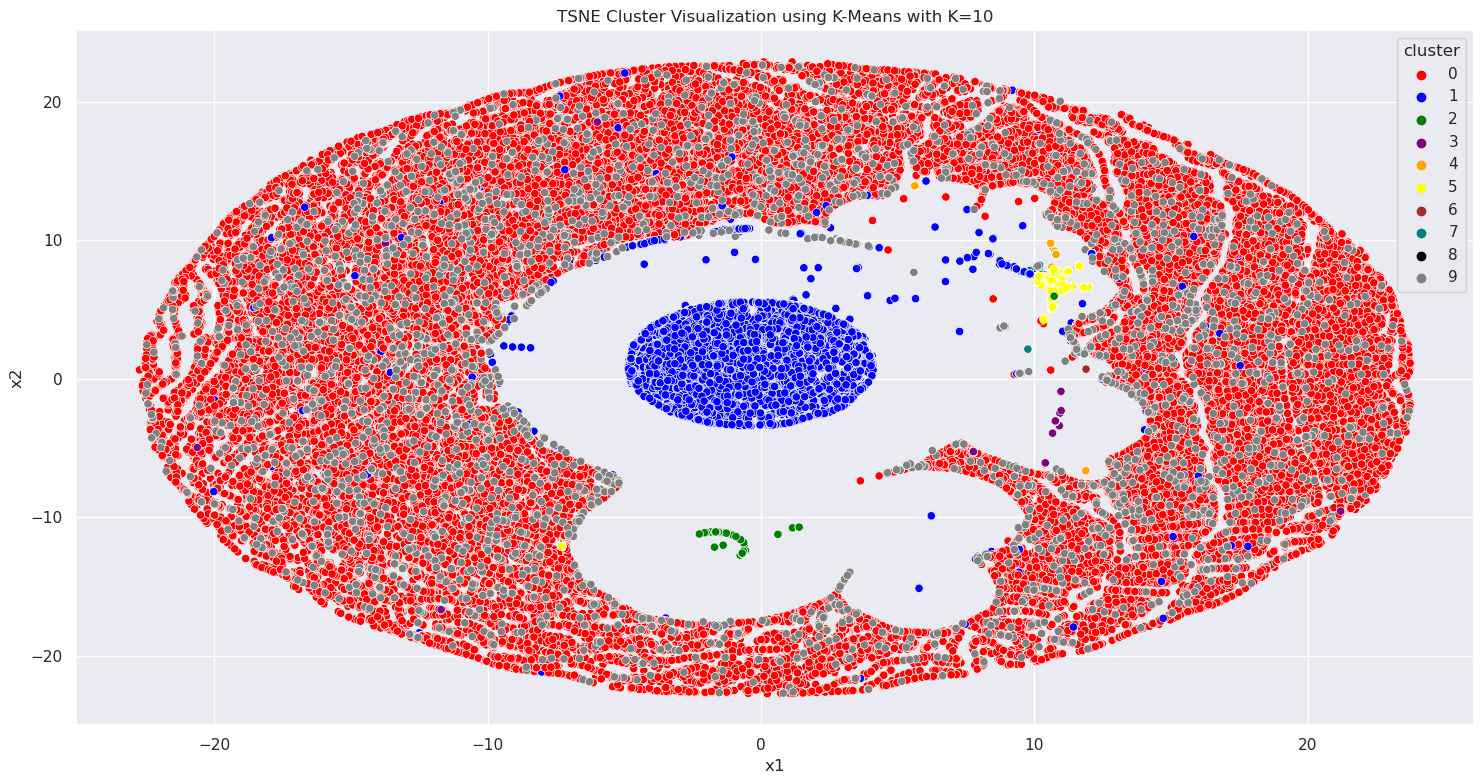
\includegraphics[width=\textwidth]{../figures/plots/section3/tsne_kmeans_clusters.png}
                \caption{t-SNE Visualization of K-Means Clusters.}
                \label{fig:tsne_kmeans}
            \end{subfigure}
            \hfill
            \begin{subfigure}[c]{0.47\textwidth}
                \centering
                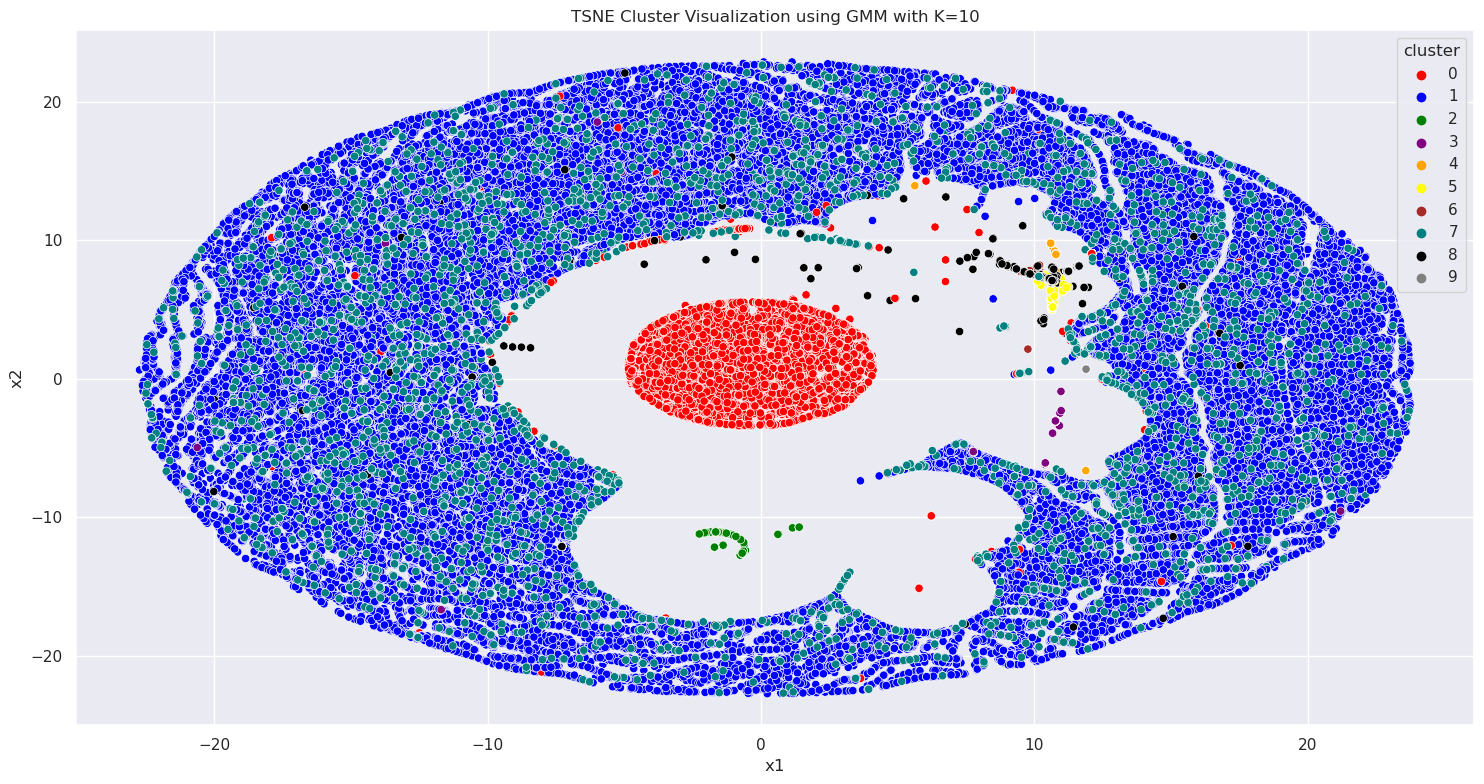
\includegraphics[width=\textwidth]{../figures/plots/section3/tsne_gmm_clusters.png}
                \caption{t-SNE Visualization of GMM Clusters.}
                \label{fig:tsne_gmm}
            \end{subfigure}
            \vspace{-0.1cm}
            \caption{}
            \label{fig:}
        \end{figure}

        \subsubsection{K-Means Visualization \\}
        
        

        \subsubsection{GMM Visualization \\}

        

    \subsection{Clusters Analysis}

        \subsubsection{Word Cloud Representation \\}

        Word clouds were generated for each cluster to highlight the most significant terms. These visualizations provided an intuitive understanding of the key features within each cluster by emphasizing frequently occurring terms. The approach helped in identifying the distinguishing characteristics of each cluster, offering insights into the behavioral patterns and intents associated with different attack sessions.

        The word clouds revealed dominant keywords for specific clusters, such as commands, parameters, or phrases frequently used in SSH attacks. This information serves as a valuable reference for understanding the nature of the clustered attack sessions, aiding in further analysis and interpretation of the underlying data.


            \begin{figure}[H]
                \centering
                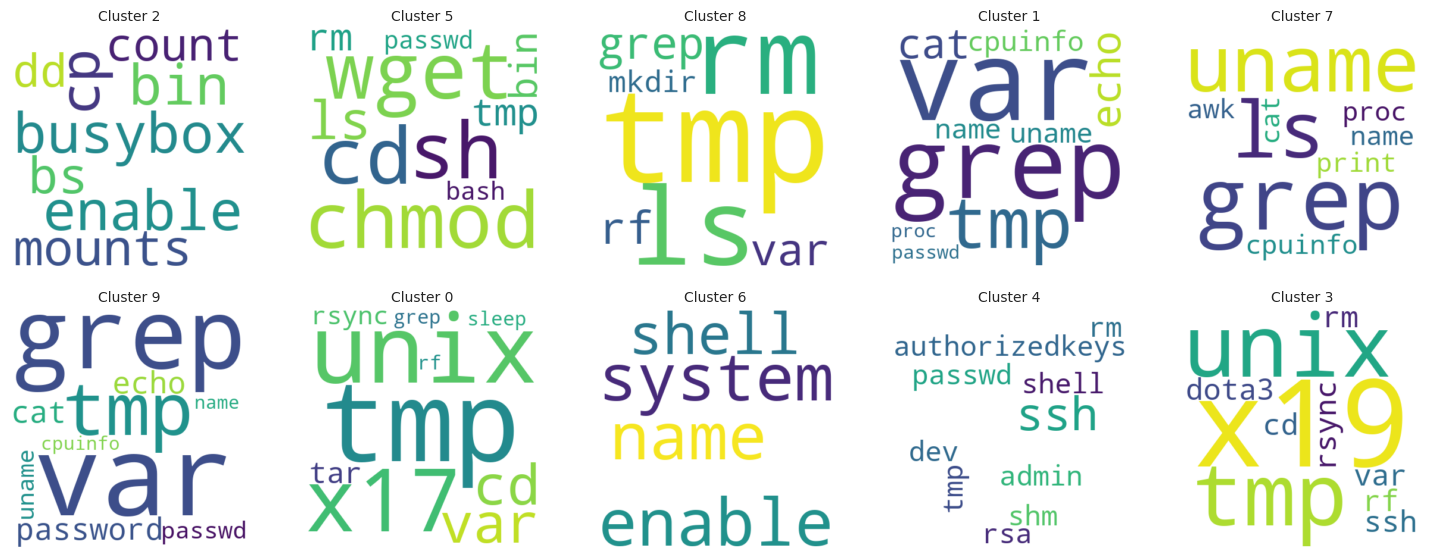
\includegraphics[width=0.9\textwidth]{../figures/plots/section3/circular_wordclouds.png}
                \caption{Word Clouds for Each Cluster.}
                \label{fig:word_clouds}
            \end{figure}

        \subsubsection{Community Detection \\}

            Graph-based community detection was performed within selected clusters to identify subgroups. This approach involves constructing a graph where nodes represent features or sessions, and edges indicate relationships or co-occurrences within the data. The Louvain method was applied to detect communities, maximizing modularity to ensure well-defined groups.

            The analysis revealed meaningful relationships and substructures within the clusters, helping to further refine the understanding of the dataset's internal patterns. These subgroups highlight finer-grained distinctions within the clusters, such as frequently occurring command sequences or behavioral traits that are common in certain attack types. Visualizations of these detected communities provide insights into the interconnectedness of the data and potential hierarchical structures in SSH attack patterns.      
        
            \begin{figure}[H]
                \centering
                \begin{subfigure}[c]{0.47\textwidth}
                    \centering
                    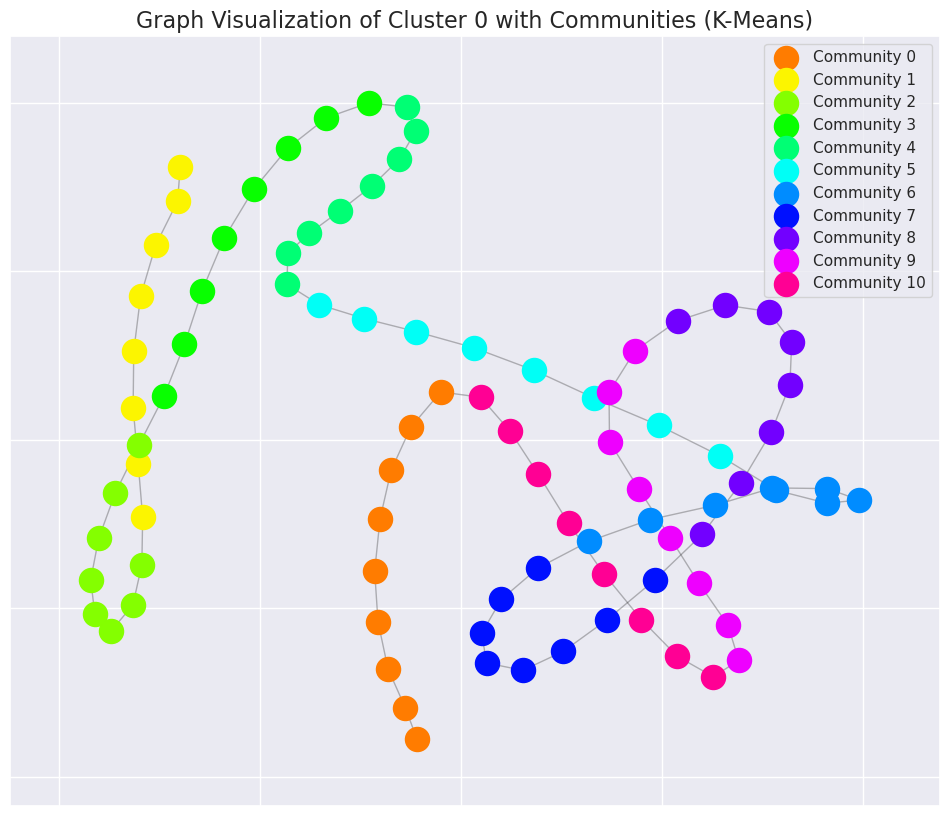
\includegraphics[width=0.8\textwidth]{../figures/plots/section3/k-means_graph_visualization_of_cluster_0_with_communities.png}
                    \caption{Community Detection in Cluster 0 (K-Means).}
                    \label{fig:kmeans_graph}
                \end{subfigure}
                \hfill
                \begin{subfigure}[c]{0.47\textwidth}
                    \centering
                    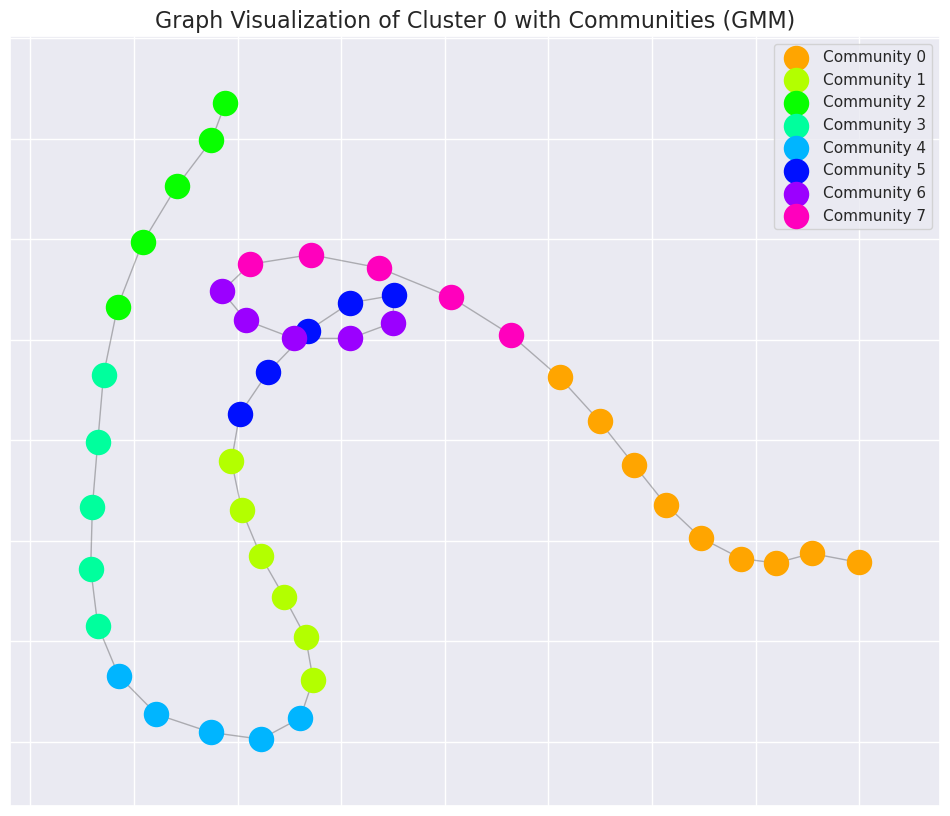
\includegraphics[width=0.8\textwidth]{../figures/plots/section3/gmm_graph_visualization_of_cluster_0_with_communities.png}
                    \caption{Community Detection in Cluster 0 (GMM).}
                    \label{fig:gmm_graph}
                \end{subfigure}
                \vspace{-0.1cm}
                \caption{}
                \label{fig:}
            \end{figure}

            % text

    \subsection{Conclusion}
    
        This analysis provided valuable insights into the patterns of SSH attacks through clustering. The K-Means and GMM algorithms both effectively identified meaningful clusters, as supported by validation metrics and visualizations. Hyperparameter tuning further enhanced the performance of both models. The results demonstrate the potential of unsupervised learning in uncovering hidden patterns in complex datasets, providing a foundation for future applications such as anomaly detection and improved cybersecurity strategies.
